\RequirePackage{hyphsubst} % Zur verbesserten Worttrennung
% Bitte an die Sprache anpassen die an \documentclass übergeben wird
	\HyphSubstLet{ngerman}{ngerman-x-latest}
	%\HyphSubstLet{english}{usenglishmax}

\documentclass[final, english, ngerman, a4paper, 10pt, % Bei Änderung der Sprache 2 x kompilieren!
numbers=noenddot,
cd=true,
cdfont=false,cdfont=nohead,cdfont=nodin,
cdmath=false,
cdhead=false,
cdfoot=true,
cdcover=monochrome,
cdgeometry=symmetric,
declaration=heading,
declaration=notoc,
abstract=heading,
]{tudscrartcl}
% final/draft
% tudscrver: Hier -- wenn bekannt -- die Versionsnummer des verwendeten tudscr-Pakets eintragen (z.B.: "tudscrver=2.05"), damit die Datei bei möglichen Änderungen auch nach einem Paketupdate ein gleichbleibendes Erscheinungsbild beibehält

\usepackage{../settings/tudbwlimPackages}
\usepackage{../settings/tudbwlimStyle}

\TUDoptions{headingsvskip=-2cm,}
\setkomafont{pagehead}{\normalfont\normalcolor\sffamily}%\slshape

\RequirePackage[breaklinks=true]{hyperref}
	\hypersetup{pdfprintscaling=None}
	\hypersetup{hypertexnames=false, colorlinks=true, linktoc=section, linkcolor=blue, citecolor=orange, urlcolor=magenta}
	
\RequirePackage[labelfont=bf, list=off]{subcaption}
\captionsetup{font=sf, labelfont=bf, labelsep=space} %textformat=period,
\captionsetup{singlelinecheck=off, format=hang, justification=raggedright}
%	\captionsetup[subfigure]{format=hang}
\captionsetup[subfloat]{labelformat=brace,list=off}
\RequirePackage{floatrow}
\floatsetup{font=sf} %
\floatsetup[table]{style=plaintop,} % font=sf

\newcommand{\pfad}[1]{{\ttfamily\glqq #1\grqq}}

\begin{document}
	
\title{Anleitung zur Verwendung der Vorlage für wissenschaftliche Arbeiten}
\author{\empty}

\date[]{\today}

%\supervisor{Dipl.-Kfm. Max Mustermann}
%\professor{Prof. Dr. Udo Buscher}
%
%%\makecover
%
%\setcounter{page}{1}
%
%%%% IM
\headlogo{../settings/IM-Logo}
\chair{Lehrstuhl für BWL, insbes. Industrielles Management, Prof. Dr. Udo Buscher}

%%% CBM
%\headlogo{../settings/CBM-Logo}
%\chair{Lehrstuhl für BWL, insbes. Industrielles Management -- Zentrum Car Business Management}

\maketitle[cdfont=false]

%\microtypesetup{protrusion=false}
%% Inhaltsverzeichnis
%\tableofcontents
%
%%% Abbildungsverzeichnis (falls nichts benötigt, einfach als Kommentar setzen)
%%\listoffigures
%%\addcontentsline{toc}{chapter}{\listfigurename}
%%
%%% Tabellenverzeichnis (falls nichts benötigt, einfach als Kommentar setzen)
%%\listoftables
%%\addcontentsline{toc}{chapter}{\listtablename}
%%
%%% Algorithmenverzeichnis (falls nichts benötigt, einfach als Kommentar setzen)
%%\listofalgorithms
%%\addcontentsline{toc}{chapter}{\listalgorithmname}
%
%\microtypesetup{protrusion=true}

\section{Benötigte Software}

Installieren Sie die folgenden Programme bitte in der dargestellten Reihenfolge. Sollten Sie nicht sicher sein auf welcher Architektur Ihr System basiert, dann installieren Sie die 32-Bit Versionen der Programme.
\begin{enumerate}
\item \href{http://www.ghostscript.com/download/gsdnld.html}{Ghostscript}\\
Postscript und PDF Interpreter

\item \href{http://pages.cs.wisc.edu/~ghost/gsview/}{Ghostgum GSview}\\
Programm zur Anzeige von Postscript-Dateien

\item \href{http://www.tug.org/texlive/acquire-netinstall.html}{TeX Live 2017}\\
Latex-Distribution (entspricht Basissystem zur Verarbeitung von Latex-Dokumenten)

\item \href{http://texstudio.sourceforge.net/}{TeXstudio}\\
Editor zur Erstellung von TeX-Dokumenten

\item \href{http://jabref.sourceforge.net/}{JabRef}\\
Programm zur Literaturverwaltung
\end{enumerate}
Zur Verwendung der Vorlage wird das \href{https://www.ctan.org/pkg/tudscr?lang=en}{tudscr}-Paket in der Version $\geq$ 2.05m benötigt.  Darüber hinaus werden die Pakete \href{https://ctan.org/pkg/biber?lang=en}{biber} und \href{https://ctan.org/pkg/biblatex?lang=en}{biblatex} in der Version $\geq$ 2.10 bzw. $\geq$ 3.10 benötigt.
Diese Pakete werden in der notwendigen Version mit TeX Live 2017 (Stand: 20. Dezember 2017) mitgeliefert, bei älteren TeX Live Distributionen werden beim Kompilieren der Vorlage Fehler auftreten! Sollten Sie TeX Live 2017 vor dem 20. Dezember 2017 installiert haben, können Sie die Pakete über den TeX Live Manager aktualisieren.



\section{Empfohlene Einstellungen für diese Vorlage}

\subsection*{TeXstudio}

Bevor Sie Änderungen vornehmen, denken Sie bitte daran Ihre aktuellen Einstellungen als Profil unter \pfad{Optionen $\rightarrow$ Profil speichern} zu speichern. Die geänderten Einstellungen können Sie dann ebenso als Profil ablegen.

Abweichend von den Standardeinstellungen muss unter \pfad{Optionen $\rightarrow$ TeXstudio konfigurieren $\rightarrow$ Erzeugen} lediglich das Standardprogramm zur Erzeugung der Bibliographie zu Biber geändert werden. Die Einstellungen sind in \autoref{fig:settings} dargestellt.
\begin{figure}[p]
	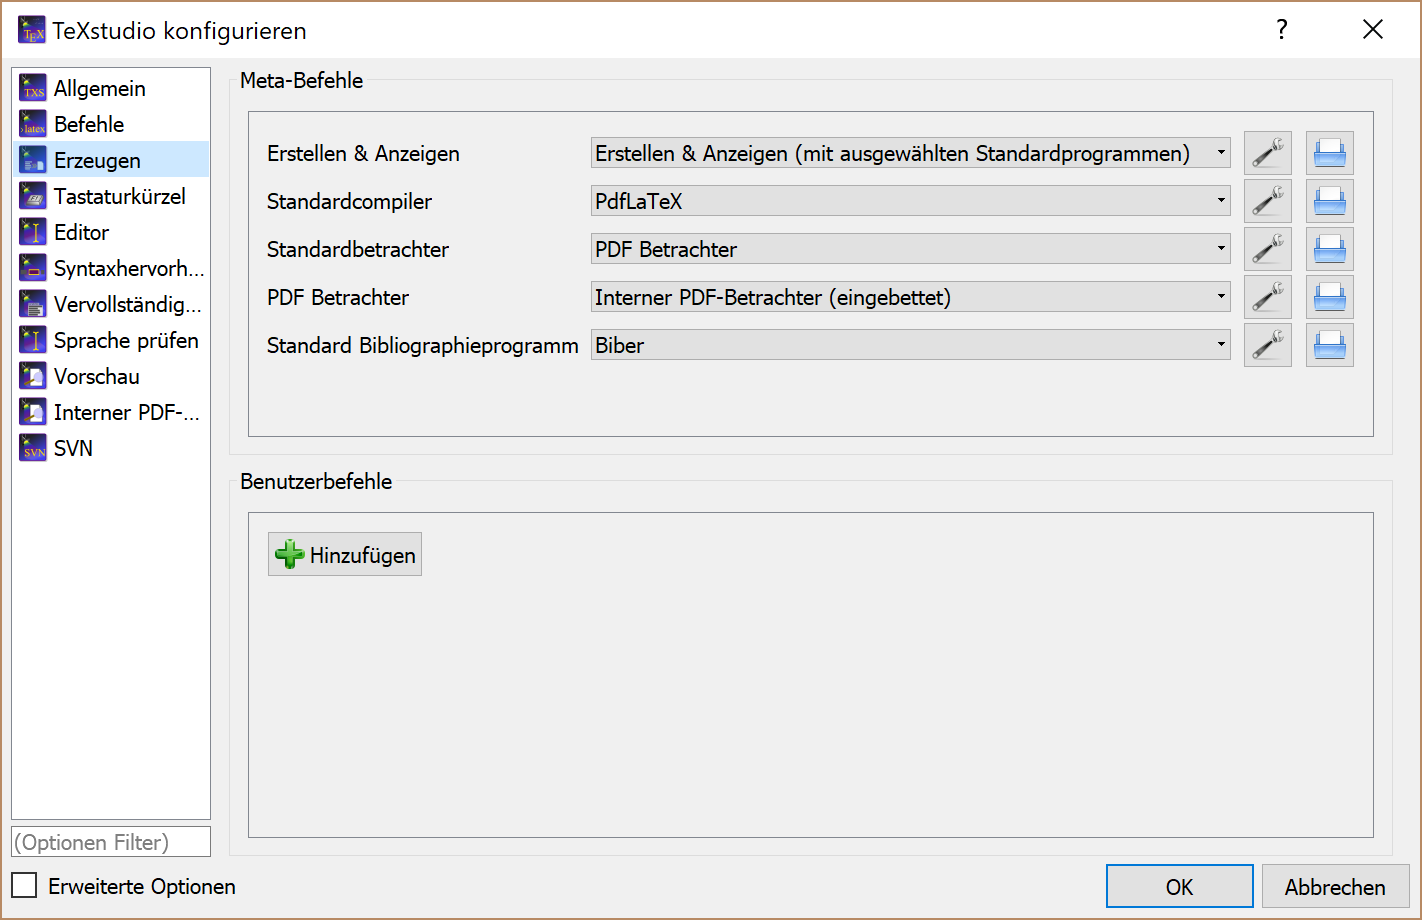
\includegraphics[width=\textwidth]{./TexStudioSettings}
	\caption{TeXstudio Einstellungen}\label{fig:settings}
\end{figure}

\subsection*{JabRef}

Unter Umständen muss im Literaturverwaltungsprogramm der Ausgabe-/Bibliographiemodus von BibTeX zu BibLaTeX geändert werden. Für JabRef ist diese Einstellung unter \pfad{Options -> Preferences -> General -> Default Bibliography Mode} zu finden. Dort sollte man auch die Zeichenkodierung zu UTF-8 ändern, siehe \autoref{fig:JabRefSettings}.
\begin{figure}[p]
	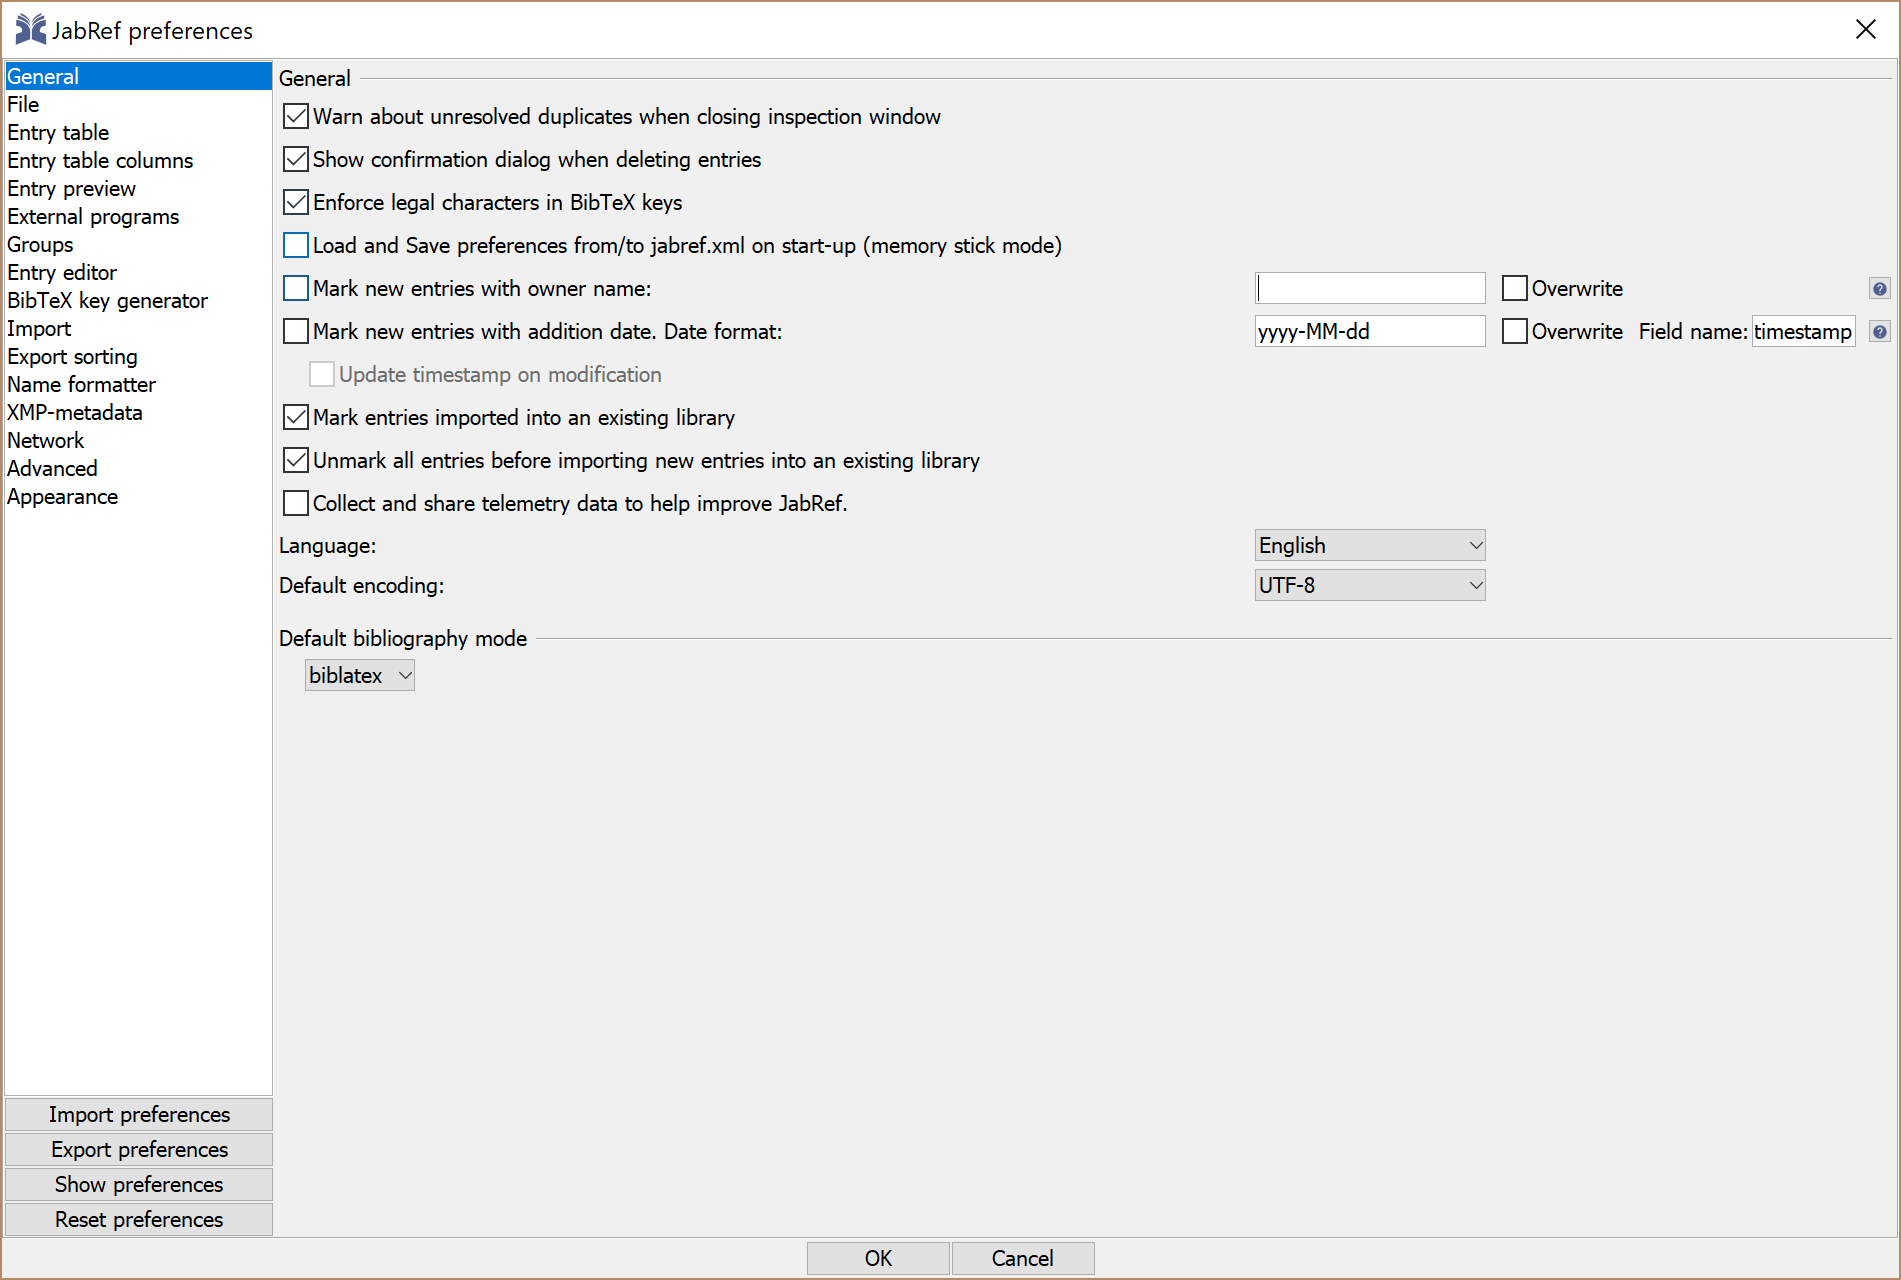
\includegraphics[width=\textwidth]{./JabRefSettings}
	\caption{JabRef Einstellungen}\label{fig:JabRefSettings}
\end{figure}



\section{Kompilierreihenfolge}

\subsection*{Erstmaliges Kompilieren}

Beim erstmaligen Erstellen der Vorlage müssen vier Schritte ausgeführt werden:\footnotemark
\begin{enumerate}
	\item PdfLaTeX
	\item Biber
	\item PdfLaTeX
	\item PdfLaTeX
\end{enumerate}
Abhängig von der Aktualität Ihrer Installation werden diese Schritte beim \enquote{Erstellen \& Anzeigen} (\texttt{F5}) automatisch ausgeführt. Ist dies nicht der Fall, führen Sie die Schritte wie oben angegeben aus. Das Bibliographieprogramm (Biber) kann dabei über das Tastenkürzel \texttt{F8} aufgerufen werden.
\footnotetext{Die nachfolgenden Tastenkürzel wurden mit TeXstudio in der Version 2.12.6 getestet.}

\subsection*{Abermaliges Kompilieren}

Soll nur der Inhalt des Dokuments aktualisiert werden, dann ist es ausreichend mit PdfLaTeX zu kompilieren:
\begin{enumerate}
	\item PdfLaTeX
\end{enumerate}
Hat sich der Inhalt der Literaturdatei (\pfad{Quellen.bib}) geändert, so muss das Bibliographieprogramm ausgeführt werden, um die Änderungen im Dokument anzuzeigen:\footnotemark
\begin{enumerate}
	\item Biber
	\item PdfLaTeX
\end{enumerate}
Normalerweise reicht auch hier \enquote{Erstellen \& Anzeigen} (\texttt{F5}).
\footnotetext{\href{https://tex.stackexchange.com/questions/154751/biblatex-with-biber-configuring-my-editor-to-avoid-undefined-citations/154754}{Dieser} und \href{https://tex.stackexchange.com/questions/153647/biblatex-biber-and-latex-citations-undefined}{dieser} Beitrag diskutieren das Problem und zeigen mögliche Lösungen auf.}


\section{Hinweise}

Eine Vorlage für das Erstellen von Präsentationen (\texttt{bwlimbeamer.tex}) und Poster für Abschlussarbeiten (\texttt{bwlimposter.tex}) wird ebenfalls bereitgestellt. Dort sind keine besonderen Einstellungen zu beachten.

Die Vorlagen basieren auf dem \href{https://www.ctan.org/pkg/tudscr?lang=en}{tudscr}-Paket von Falk Hanisch. Die zugehörige Paketdokumentation ist äußerst verständlich und detailliert geschrieben, besonders zu empfehlen ist das \href{http://mirrors.ctan.org/macros/latex/contrib/tudscr/doc/tudscr.pdf}{Benutzerhandbuch} und der \href{http://mirrors.ctan.org/macros/latex/contrib/tudscr/doc/tutorials/treatise.pdf}{Anwenderleitfaden}.
Weitere nützliche Links:
\begin{itemize}
	\item \href{https://github.com/tud-cd/tudscr}{GitHub-Seite des TUD-Script-Bundle}
	\item \href{https://latex.wcms-file3.tu-dresden.de/phpBB3/}{TU Dresden LaTeX Forum}
	\item \href{http://wwwpub.zih.tu-dresden.de/~fahan/tudscr/index.php}{Installationsskripte für die Schriften des Corporate Design}
	\item \href{https://tu-dresden.de/bu/wirtschaft/lim/studium/abschlussarbeiten}{Abschlussarbeiten am Lehrstuhl Industrielles Management}
\end{itemize}
	
\end{document}